\documentclass[13pt, t]{beamer}

% Presento style file
\usepackage{config/presento}

% custom command and packages
% custom packages
\usepackage{textpos}
\setlength{\TPHorizModule}{1cm}
\setlength{\TPVertModule}{1cm}

\newcommand\crule[1][black]{\textcolor{#1}{\rule{2cm}{2cm}}}



% Information
\title{\huge Компьютерная лингвистика...}
\subtitle{...и то, что вы ошибочно ею не считали}
\author{Г. Мороз \bigskip}
\institute{Лаборатория  языковой конвергенции, НИУ ВШЭ\\
Школа лингвистики НИУ ВШЭ}
\date{\begin{center} 
\large 2 февраля 2018, 19:00 \bigskip \\ {\color{colorblue} \href{http://znanie.vdnh.ru/events/georgiy-moroz-lingvistika-i-to-chto-vy-oshibochno-ey-ne-schitali}{Знание. ВДНХ}} \end{center}}

\begin{document}

\begin{frame}[plain]
\maketitle
\end{frame}

% \framecard[colorblue]{{\color{colorwhite} \huge Акустические меры}}

\begin{frame}{\#тыжлингвист}
\begin{itemize}
\item  \pause умеет читать на всех письменностях мира
\item знает все языки на свете
\item умеет распознавать каждый язык на слух \pause
\item может рассказать о происхождении каждого слова \pause
\item пишет без ошибок и знает все правила орфографии \pause
\item не знает математики и программирования \pause
\end{itemize}
\Large все вышеперечисленное, конечно, не правда
\end{frame}

\begin{frame}{Лингвистика}
\begin{itemize}
\item прескриптивная \pause
\item вся остальная
\begin{itemize}
\item исследования грамматики языка и языкового разнообразия
\item исследования распределения грамматических особенностей в языках мира
\item исследования когнитивных способностей человека и других животных, связанных с языком
\item исследования в области NLP и их приложения
\item исследования в области синтеза и распознования речи и языка
\item создание компьютерных инструментов для решения самых разных задач
\end{itemize}
\end{itemize}
\vfill
Еще бывает \textit{компьютерная лингвистика}, но это обобщенный термин, которым объединяют совсем несвязанные области:
\begin{itemize}
\item вспомогательные инструменты лингвистического исследования и документации
\item Computational linguistics
\item NLP
\end{itemize}
\end{frame}


\framecard[colorblue]{{\color{colorwhite} \huge Корпус текстов}}

\begin{frame}{корпус}
\begin{itemize}
\item корпус литературных текстов
\item \href{http://ruscorpora.ru/}{\color{colorblue} Русский национальный корпус}
\item аудио и видео корпуса \pause
\begin{itemize}
\item настоящая речь, а не тексты
\item см., например, \href{http://rsl.nstu.ru}{\color{colorblue} корпус русского жестового языка}
\item см., например, \href{https://www.youtube.com/watch?v=OUwOvF7TqgA&feature=youtu.be&t=1m25s}{\color{colorblue} Уошо}
\end{itemize}
\end{itemize}
\end{frame}

\begin{frame}{корпус: дневник Марты Баллард}
Марта Баллард, акушерка из штата Мэн, которая вела дневник с 1785 по 1812 год\\
{\tiny http://www.cameronblevins.org/posts/topic-modeling-martha-ballards-diary/}
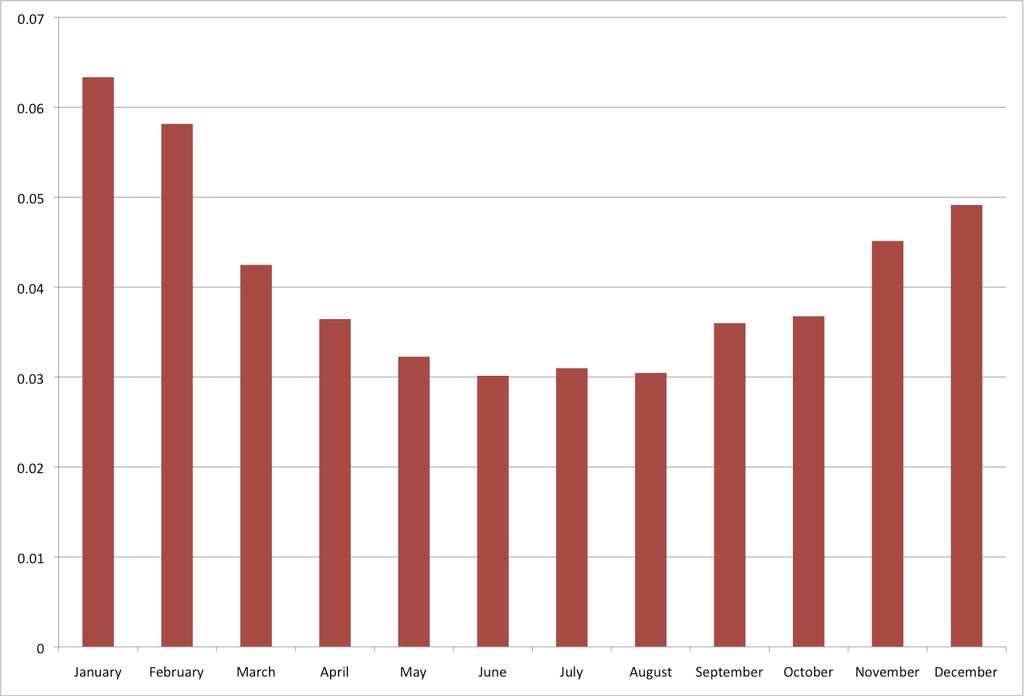
\includegraphics[width=0.8\linewidth]{images/01-ballard}\\
\pause
Холодная погода
\end{frame}

\begin{frame}{корпус: дневник Марты Баллард}
Марта Баллард, акушерка из штата Мэн, которая вела дневник с 1785 по 1812 год\\
{\tiny http://www.cameronblevins.org/posts/topic-modeling-martha-ballards-diary/}
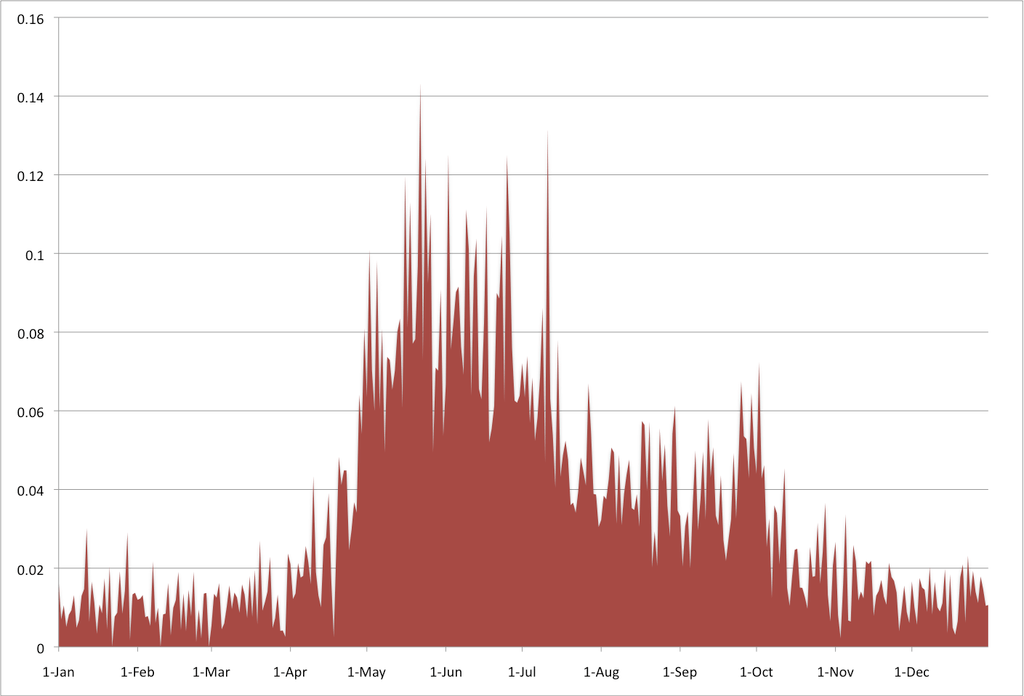
\includegraphics[width=0.8\linewidth]{images/02-ballard}\\
\pause
Работы в саду
\end{frame}

\begin{frame}{корпус: \href{https://books.google.com/ngrams}{Google ngrams}}
Google оцифровали примерно 15 млн. книг и положили 5 млн. в Google Books:\\
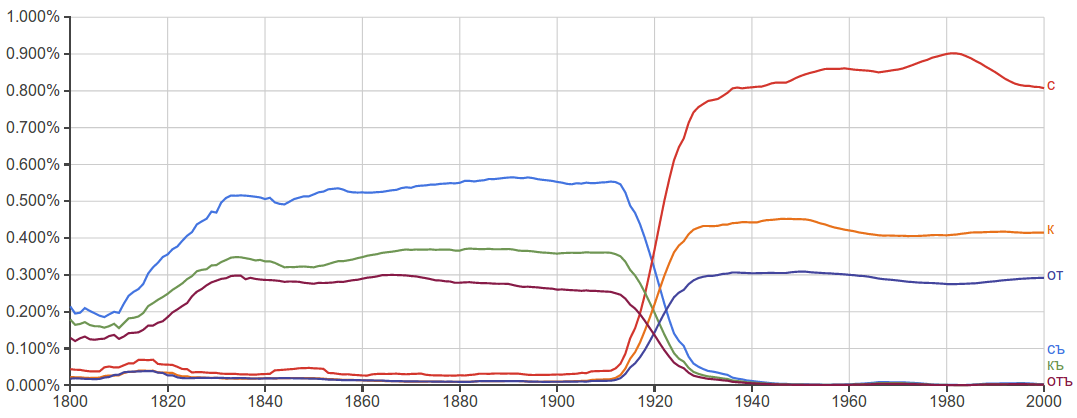
\includegraphics[width=\linewidth]{images/03-google-ngrams}\\
Казалось бы хорошая штука, но русские лингвисты ею не пользуются...
\end{frame}

\begin{frame}{корпус: \href{https://books.google.com/ngrams}{Google ngrams}}
Google оцифровали примерно 15 млн. книг и положили 5 млн. в Google Books:\\
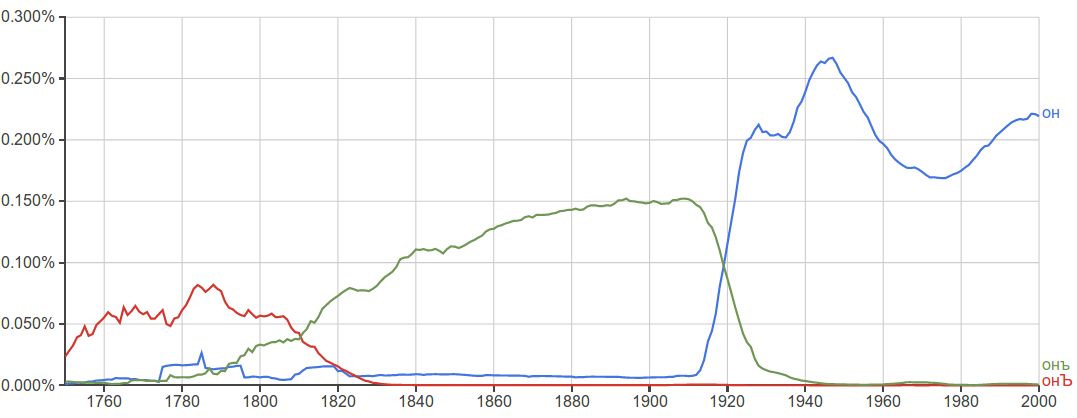
\includegraphics[width=\linewidth]{images/04-google-ngrams}\\
Казалось бы хорошая штука, но русские лингвисты ею не пользуются...
\end{frame}

\begin{frame}{корпус: \href{http://ruscorpora.ru/}{\color{colorblue} Русский национальный корпус}}
\href{http://ruscorpora.ru/}{\color{colorblue} Русский национальный корпус} сделан лингвистами, для лингвистов 
\end{frame}

\framecard[colorblue]{{\color{colorwhite} \huge Natural Language Processing}}

\begin{frame}{Natural Language Processing}
\begin{itemize}
\item оптическое распознавание символов
\item распознавание и синтез речи
\item анализ текста, анализ тональности текста
\item машинный перевод
\item чатботы
\item спеллчекеры
\item ...
\end{itemize}
\end{frame}

\framepic{images/05-ocr-translater.jpeg}

\framepic{images/06-alisa.jpg}


\framecard[colorblue]{{\color{colorwhite} \huge Спасибо за внимание! \bigskip\\
\Large Пишите письма\\
agricolamz@gmail.com}}

\end{document}